\documentclass[../phys-f308.tex]{subfiles}

\begin{document}
    \part{Solids and liquids - Viscoelasticity}

    \begin{abstract}
        The goal is to provide a description of the behavior of viscoelastic materials. To do so we will exploit the Maxwell model
    \end{abstract}


    \section{Response of a material to shear stress}

    \begin{definition}[For solids]
        Stress is the force applied to a material, divided by the material's section area. Concretely, it is given by
        \begin{equation}
            \sigma = \frac{Force}{Area}
        \end{equation}
    \end{definition}

    \begin{definition}
        The shear strain is the deformation or displacement resulting from the application of a force.
        \begin{align}
            e &= \frac{\Delta x}{y}\\
            e_{xy} &= \frac{\partial u_x}{\partial y}+\frac{\partial u_y}{\partial x}
        \end{align}
        where $u_i$ is the displacement along the direction $i$.
    \end{definition}

    \begin{property}
        Many material exhibit a proportionnal relationship between stress and strain up to a certain point.\\
        
        For solids,
        \begin{equation}
            \sigma_{xy} = G_\infty e_{xy}
        \end{equation}
        where $G_\infty$ is the shear modulus.\\

        For a Newtonian liquid,
        \begin{equation}
            \sigma_{xy} = \eta\frac{v}{h} = \eta\left(\frac{\partial v_x}{\partial y}+\frac{\partial v_x}{\partial x}\right) = \eta\dot{e}_{xy}
        \end{equation}
        where $\eta$ is the shear viscosity.
    \end{property}

    The simplest method to characterize the dynamic behaviour of a material is to study its time respond to an excitation given by the Heaviside function at \textbf{small forces/disturbances} (in the linear regime). Then,

    \begin{equation}
        G(t) = \frac{1}{e_o}\sigma(t) \quad J(t) = \frac{1}{\sigma_0}e(t)
    \end{equation}


    The response of an ideal elastic solid (spring) may be written as
    \begin{equation}
        e = \frac{\sigma}{G_\infty}
    \end{equation}
    Similarly for a Newtonian liquid (damper), one has
    \begin{equation}
        \frac{\partial e}{\partial t} = \frac{\sigma}{\eta}
    \end{equation}

    \subsection{Spring in series with damper}

    Let us put a spring in series to a damper. In such a situation the deformation is the sum of the deformations in the single elements and the same stress is applied to each element.

    \begin{equation}
        \begin{cases}
            e &= e_G+e_\eta\\
            \sigma &= \sigma_G+\sigma_\eta
        \end{cases}
        \label{eq: spring in series to a damper}
    \end{equation}

    In this expression, $\sigma$ is similar to the intensity of a current in an electrical circuit with resistances $e$ in series.\\

    From \eqref{eq: spring in series to a damper}, one has that
    \begin{equation}
        \dot{e} = \dot{e}_G+\dot{e}_\eta
    \end{equation}
    For the elastic solid (spring), $\dot{e}_G = \frac{\dot{\sigma}}{G_\infty}$. For the Newtonian liquid (damper), $\dot{e}_\eta = \frac{\sigma}{\eta}$. Hence,
    \begin{equation}
        \dot{e} = \frac{\dot{\sigma}}{G_\infty}+\frac{\sigma}{\eta}\\
        \frac{\partial e}{\partial t} = \frac{1}{G_\infty}\frac{d\sigma}{dt}+\frac{\sigma}{\eta}
    \end{equation}

    In a relaxation experiment, one applies an instataneous constraint and observes how the stress evolves at \textbf{constant constraint}.\\

    \begin{property}
        Let us study how the system would relax upon the application of an instantaneous constant constraint $e_0$ at $t=0$ when $\sigma=0$.
        \begin{equation}
            \frac{\partial e}{\partial t} = \frac{1}{G_\infty}\frac{d\sigma}{dt}+\frac{\sigma}{\eta}=0\quad\Rightarrow\quad\sigma(t)=e_0G_\infty\exp\left(-\frac{t}{\eta}G_\infty\right)\quad\Rightarrow\quad G(t)=G_\infty\exp\left(-\frac{t}{\eta}G_\infty\right)
        \end{equation}
        En posant $\tau = \frac{\eta}{G_\infty}$, nous pouvons réécrire
        \begin{equation}
            G(t) = G_\infty\exp\left(-\frac{t}{\eta}\right)
        \end{equation}
    \end{property}

    \subsection{Viscoelasticity}

    \begin{definition}
        The Deborah number is the ratio between $\tau$ and the observation time.
        \begin{equation}
            De = \frac{\tau}{t_{obs}}
        \end{equation}
    \end{definition}

    For short observation times ($t<<\tau$), materials tend to have a solid-like behavior ($De>>1$) whereas with long observation-times ($t>>\tau$) there will be a liquid-like behavior ($De<<1$).

    \begin{definition}
        Real materials behave like solids at short observation times and like liquids at long observation times.
    \end{definition}

    \section{Flucutation dissipation theorem}

    \begin{definition}[Onsanger regression hypothesis]
        The relaxation of macroscopic non-equilibrium disturbance is governed by the same laws as the regression of spontaneous microscopic fluctuations in an equilibrium system.
    \end{definition}

    \begin{theorem}[FDT]
        At thermodynamic equilibrium the response of a system to an outer disturbance within the linear regime is related to the spontaneous fluctuations of the system.
    \end{theorem}

    Therefore, \emph{the relaxation times we measure in the linear regime and at thermodynamic equilibrium are the characteristic times of the spontaneous fluctuations of the system.}

    From the FDT one has that the macroscopic response of a system to a force $\bm{F}$ (meaning $\tau$) is also associated to the characteristic relaxation time relative to the spontaneous fluctuations. $\tau$ thus indicates the effective characteristic time of the system in the absence of external perturbations.\\

    \section{Temperature dependance of the timescale of molecular mobility}

    Neighbors impose a 'cage', i.e a potential barier $\epsilon$. In this view, the relaxation time is the time necesaary to jump out of the cage. This follows a Boltzmann distribution
    \begin{equation}
        \tau\sim\exp\left(\frac{\epsilon}{k_BT}\right)
    \end{equation}

    Atoms//molecules vibrate at a characteristic frequency $\nu$.

    \begin{equation}
        \tau = \nu^{-1}\exp\left(\frac{\epsilon}{k_BT}\right)
    \end{equation}

    In the case of liquids supercooled below the melting point, a phenomenological expression for $t$ is given by the \emph{Vogel Fulcher Tamman} equation
    \begin{equation}
        \tau = \tau_\infty\exp\left(\frac{A}{T-T_0}\right)
    \end{equation}

    \part{Solids and liquids: the glass transition}

    \begin{abstract}
        In order to understand the glass transition, we shall:
        \begin{itemize}
            \item Determining the temperature dependence of the crystalization rate ;
            \item Identifying the conditions permitting to solidify while avoiding the formation of crystals ;
            \item Describing the temperature dependence of volume in equilibrium and nonequilibrium conditions.
        \end{itemize}
    \end{abstract}

    \section{Molecular picture}

    To grow crystals, a nucleus must first be formed. Then, more and more molecules/atoms diffuse and get attached to the nucleus.\\

    In the condensed phase molecules oscillate withing the cage formed by their neighbors. Diffusion is then given by the probability to escape from the cage and to jump in a vacancy. The formation of the vacancy has a well finite probability.

    \begin{equation}
        t_D = t_{cage}+t_{jump} \approx t_{cage}
    \end{equation}

    singe $t_{cage}>>t_{jump}$.

    \begin{property}
        The probability for a diffusion to occur is given by 
        \begin{equation}
            D(T) = D_0\exp\left(-\frac{\Delta W}{k_BT}\right)
        \end{equation}
    \end{property}
    \begin{proof}
        The probability $P_0$ to overcome an energy barrier $\Delta G_0$ is calculated via a Boltzmann distribution.

        \begin{equation}
            P_0 = C\exp\left(-\frac{\Delta G_0}{k_BT}\right) = C\exp\left(-\frac{\Delta H_0}{k_BT}+\frac{\Delta S_0}{k_B}\right) = \tilde{C}\exp\left(-\frac{\Delta W}{k_BT}\right)
        \end{equation}
        Taking into account the probability to form a vacancy $\Delta G_{vac}$, one has
        \begin{equation}
            P_{vac} = \bar{C}\exp\left(-\frac{\Delta H_{vac}}{k_BT}\right)
        \end{equation}
        Then,
        \begin{equation}
            P_{diff} = P_0P_{vac} = C\exp\left(-\frac{\Delta H_0+\Delta H_{vac}}{k_BT}\right) = C\left(-\frac{\Delta W}{k_BT}\right)
        \end{equation}
        Let us notice that this is a thermically acticated process. $\Delta W$ depends on the type of barrier and the mechanism considered.
    \end{proof}

    \subsection{Crystallization rate}

    \begin{property}
        The crystalization requires both nucleation and growth (diffusion).

        \begin{equation}
            I = \frac{dN}{dt}\approx A\exp\left(-\frac{\Delta G_{diff}}{kT}\right)\exp\left(-\frac{\Delta G_n}{kT}\right)
        \end{equation}
        where the two exponentials have a different temperature dependence.\\

        The crystalization rate shows a maximum.
    \end{property}

    \subsection{Time-Temperature-Transformation diagram}

    \begin{figure}
        \begin{centering}
            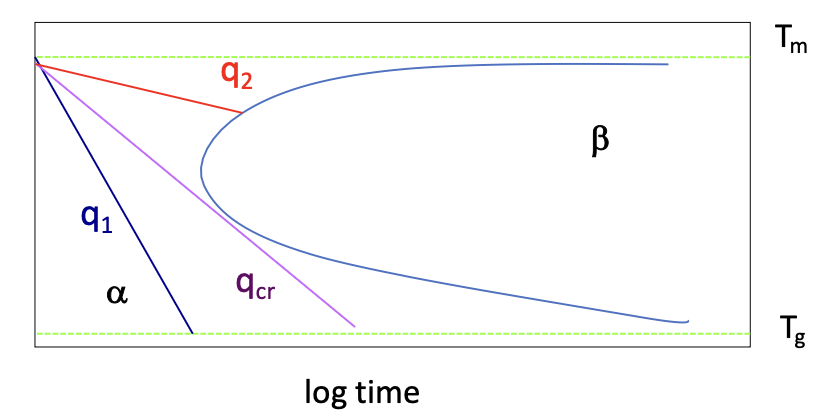
\includegraphics{Pictures/Cooling_rates.png}
            \caption{In this graph there are two states $\alpha$ and $\beta$. The top of the graph corresponds to the melting point $T_m$ and the bottom to the glass transition temperature $T_g$. For different cooling rates, one observes a different macroscopic result. For $q_1$ one has a glass transition whereas $q_{cr}$ is the critical point and $q_2$ has an $\alpha-\beta$ transition.}
        \end{centering}\label{fig: TTT}
    \end{figure}

    To estimate the critical cooling rate, we therefore need to obtain an expression for the kinetics of the phase transition.

    \section{Solidification without crystalization}

    If cooled fast enough, one can avoid the nucleation and go straight into the glass phase. This is the cooling-rate $q_1$ in $\ref{fig: TTT}$. Another way to represent this is as displayed in $\ref{fig: SHCR}$

    \begin{figure}
        \begin{centering}
            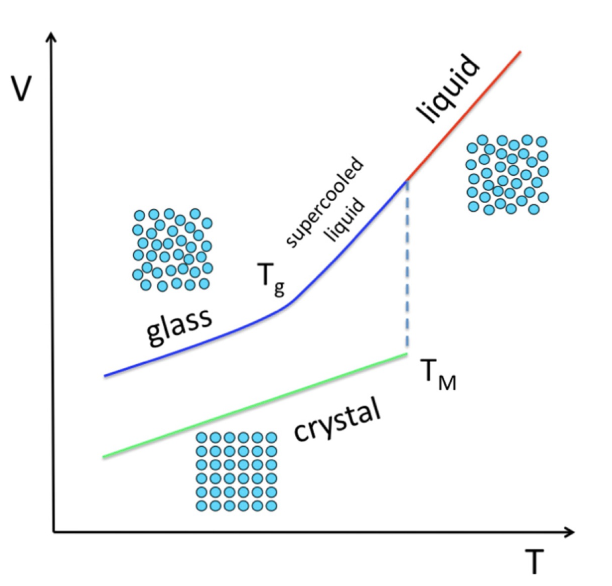
\includegraphics[width=50mm]{Pictures/Solidification_high_cooling_rates.png}
            \caption{When cooled fast-enough, the liquid turns into glass in a special glass-transition.}
        \end{centering}\label{fig: SHCR}
    \end{figure}

    \color{red} To be completed.\color{black}

    \part{Polymer physics}

    A polymer is a long molecule made up of a certain amount of a repeating unit called monomer. In this course, we consider polymers with about $10^10$ monomers, each of dimensions $1cm$.\\

    The maximum extension of an ideal chain is given by an
    \begin{equation}
        R_{max} = nl\cos\frac{\theta}{2}
    \end{equation}
    where $n$ is the polymerization degree\footnote{ie, the number of monomers.}, $l$ is the bound length and $\theta$ is the bound angle. In what cases is this conformation possible?

    \section{Conformations of an ideal chain}

    \begin{definition}
        An ideal chain is like an ideal gas: it has no net (whether repulsive or attractive) long range interactions amongst the $n$ monomers, separated by a constant bound distance $l$.
    \end{definition}

    The $n$ joint monomers are joined together to form an $R_n$ end-to-end vector.

    \begin{equation}
        \bar{R_n} = \sum_{i=1}^n\bar{r_i}
    \end{equation}
    If all the angles are random, then we have that $\langle\bar{R_n}\rangle = 0$.\\

    \color{red}\textbf{Will be compelted later on.}\color{black}

    \part{Liquid crystals}

\end{document}